\section{Methodology}
\label{sec:method}

This chapter describes the classification and similarity-scoring pipeline adapted from \citet{Nicolas2025} for the extended-source sample introduced in Chapter~\ref{sec:data}. We first learn image representations through SimCLR pre-training with random structural views, then use PCA, HDBSCAN, visual inspection and SI-SSIM filtering to construct eleven morphology classes (Secs.~\ref{sec:method_simclr}--\ref{sec:method_labels}). These labels support supervised fine-tuning of a 50-member ensemble (Sec.~\ref{sec:method_classifier}), whose probabilities and uncertainty measures define the similarity-to-radio-galaxy score \(S_\mathrm{RG}\) (Sec.~\ref{sec:method_srg}). We then establish the external-label mappings and evaluation metrics used to compare classifications (Sec.~\ref{sec:method_external_mapping}). Finally, we describe the masking and preprocessing of selected radio-relic cutouts to examine the ensemble's response to diffuse emission (Sec.~\ref{sec:method_relics}).

\subsection{Model Pre-training}
\label{sec:method_simclr}

The SimCLR framework with RSV introduced in Sec.~\ref{sec:bg_ssl} was implemented using the GreyResNet18 architecture.
GreyResNet18 is a ResNet-18 \citep{He2016} adapted for single-channel input, with its classification layer removed and
an input batch-normalisation (BN) layer whose affine parameters are disabled. Each \(128 \times 128\) cutout is mapped to a \(512\)-dimensional representation.
The projection head maps this representation through a \(512\)-dimensional linear layer, BN, and a rectified linear unit (ReLU), followed by a linear map to \(256\) dimensions.
The detailed architecture is shown in Appendix~\ref{app:greyresnet18_architecture}.

For each source, the augmentation pipeline independently generated two views using a random rotation through a continuous angle, a random vertical flip,
brightness jitter with a factor between \(0\) and \(1.1\), and a random resized crop retaining between \(90\,\%\) and \(100\,\%\) of the image area.
RSV subsequently modified the pool of second views before the positive pairs were passed to the encoder.

\paragraph{Random structural view via SI-SSIM.}
The semi-invariant structural similarity (SI-SSIM) between two images is the maximum structural similarity index \citep[SSIM;][]{Wang2004} obtained over the eight square-image symmetry transforms of the second image: rotations by multiples of \(90^{\circ}\), with and without a reflection. This construction is invariant to those eight transforms, rather than to arbitrary orientations, while preserving sensitivity to image structure. SI-SSIM is not scale invariant. A symmetric SI-SSIM matrix is precomputed once from cutouts downsampled to \(64 \times 64\) pixels and is reused for both RSV and the label-construction procedure of Sec.~\ref{sec:method_labels}.

For a source \(i\), the stored matrix is first restricted to the current minibatch and sorted by decreasing SI-SSIM. The implemented candidate set is

\[
\mathcal{C}_i=\{i,n_{i,1},n_{i,2},n_{i,3}\}, \qquad |\mathcal{C}_i|=k_{\mathrm{RSV}}=4.
\]

The first candidate is the original source because the matrix diagonal is one. The remaining three candidates are different sources in the minibatch rather than augmentations of the query.
One candidate is drawn uniformly, and the query's second augmented view is replaced by the independently augmented second view associated with that candidate.
Selecting the self-candidate therefore retains a standard same-source SimCLR pair, whereas selecting one of the other three candidates forms a cross-source positive pair. The nominal probability of forming a cross-source pair is \((k_{\mathrm{RSV}}-1)/k_{\mathrm{RSV}}=3/4\). Figure~\ref{fig:simclr_rsv_schematic} illustrates this selection rule and the shared SimCLR path.
\begin{figure}[H]
  \centering
  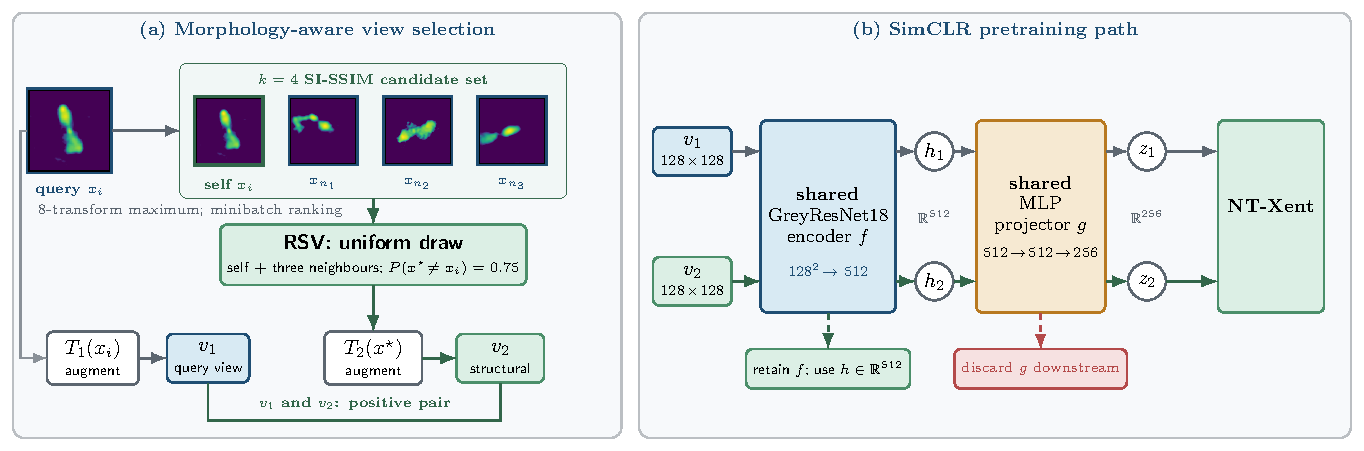
\includegraphics[width=\linewidth]{img/simclr_rsv_schematic.pdf}
  \caption[SimCLR pre-training with random structural views]{SimCLR pre-training with random structural views (RSV), adapted
    conceptually from \citet{Nicolas2025}. (a) RSV uses an independently
    augmented view of either the query or one of its three nearest SI-SSIM
    neighbours in the minibatch as the second view. (b) Both views pass through
    the shared encoder \(f\) and projector \(g\). NT-Xent is evaluated in the
    \(256\)-dimensional projection space; the \(512\)-dimensional encoder
    representation is retained downstream.}
  \label{fig:simclr_rsv_schematic}
\end{figure}

The encoder and projector were trained for \textbf{\(205\) epochs} with a \textbf{batch size of \(512\)}, AdamW \citep{Loshchilov2019}, a base \textbf{learning rate of \(3\times10^{-4}\)}, and a \textbf{weight decay of \(10^{-4}\)}. A five-epoch linear warm-up was followed by cosine annealing to one fiftieth of the base rate; training used mixed-precision arithmetic and gradient clipping at unit norm. The projection head was discarded after pre-training, and all downstream steps used the \(512\)-dimensional encoder representations.

\citet{Nicolas2025} report that removing RSV prevented the recovery of one-third of the reported morphology classes. We therefore applied RSV directly without independently assessing its effect.

The encoder and projection head were optimised with the NT-Xent objective defined in Eq.~\ref{eq:ntxent}.
Its temperature, \(\tau=0.15\), was selected empirically from a sweep of twenty runs spanning \(0.05\)--\(1.05\).
Model selection jointly favoured runs that required more principal components to retain \(90\,\%\) of the representation variance,
produced more HDBSCAN clusters, and assigned fewer sources to noise.
The selected run retained \textbf{\(15\) components}, yielded \textbf{\(59\) non-noise clusters}, and assigned \(27\,275\) sources to the noise label.

For the clustering-based evaluation described above, the \(\ell_2\)-normalised representations of all \(32\,514\) pre-training sources were reduced by
principal component analysis \citep{Jolliffe2016}. HDBSCAN \citep{Campello2013,McInnes2017} was then applied with a minimum cluster size of \(19\),
a minimum-samples value of \(1\), and the Manhattan metric. Of the full sample, \(5\,239\) sources (\(16.1\,\%\)) received non-noise labels.
The non-noise cluster sizes range from \(19\) to \(1\,502\) sources and are strongly imbalanced (Figure~\ref{fig:hdbscan_cluster_distribution}).
The three largest clusters, labels 52, 55, and 58, contain \(3\,273\) sources, or \(62.5\,\%\) of all non-noise memberships.
\begin{figure}[H]
  \centering
  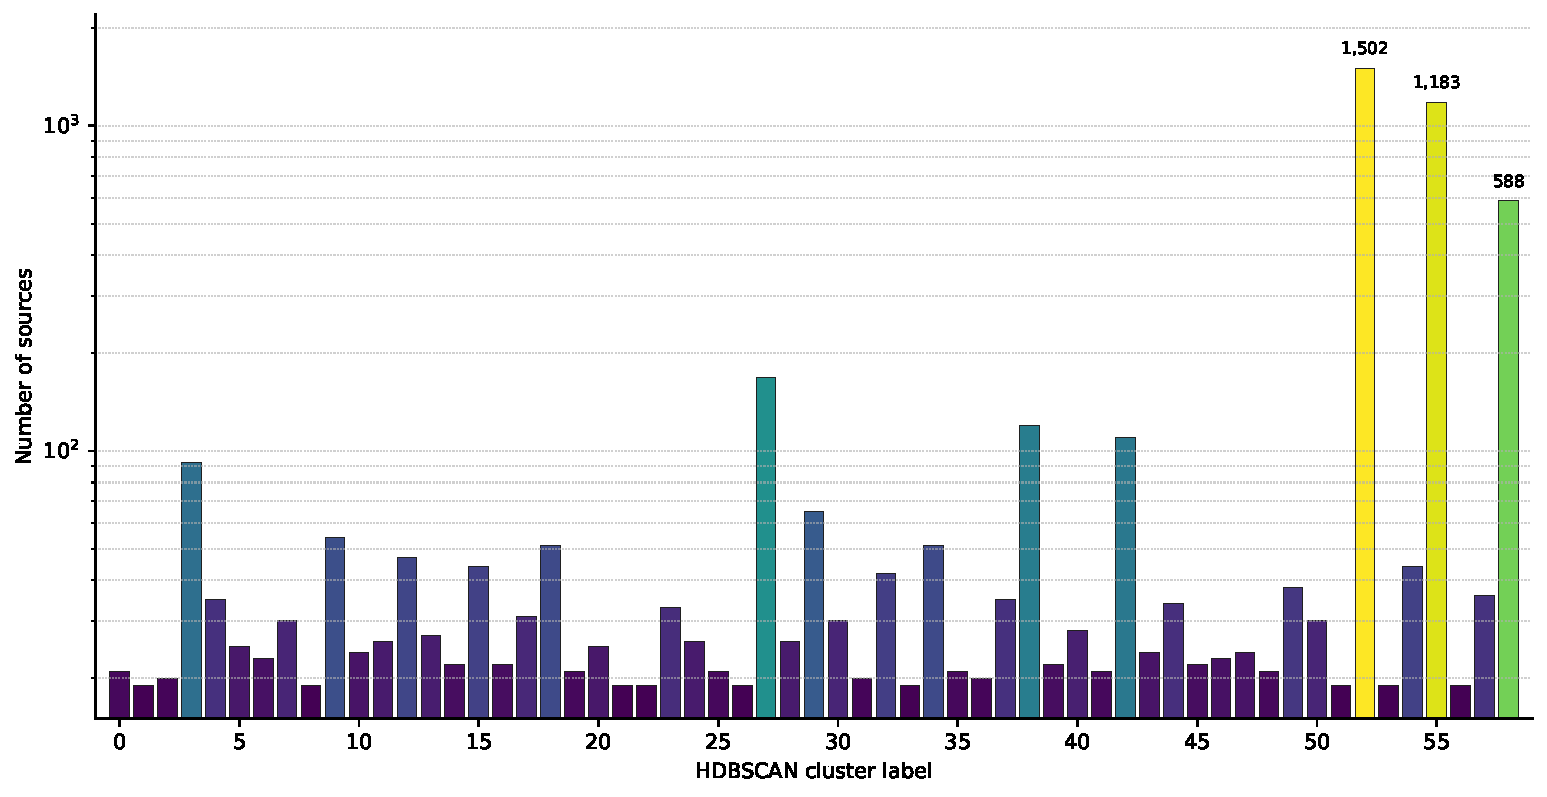
\includegraphics[width=0.85\linewidth]{img/hdbscan_cluster_distribution.pdf}
  \caption[HDBSCAN cluster membership distribution]{Membership of the 59 non-noise HDBSCAN clusters obtained using the 15 principal components that retain 90\,\% of the variance. The vertical axis is logarithmic, and the colour scale
encodes cluster size.}
  \label{fig:hdbscan_cluster_distribution}
\end{figure}

Figure~\ref{fig:hdbscan_cluster_examples} shows four randomly drawn members from six raw clusters, selected to illustrate the range of compact, elongated, bent,
and multi-component structures. These (pre-)labels denote density-based groups in the learned representation space rather than physical morphology classes.
The complete raw-cluster overview, including the noise group (cluster label -1), is provided in Appendix~\ref{app:hdbscan_cluster_overview}.
\begin{figure}[H]
  \centering
  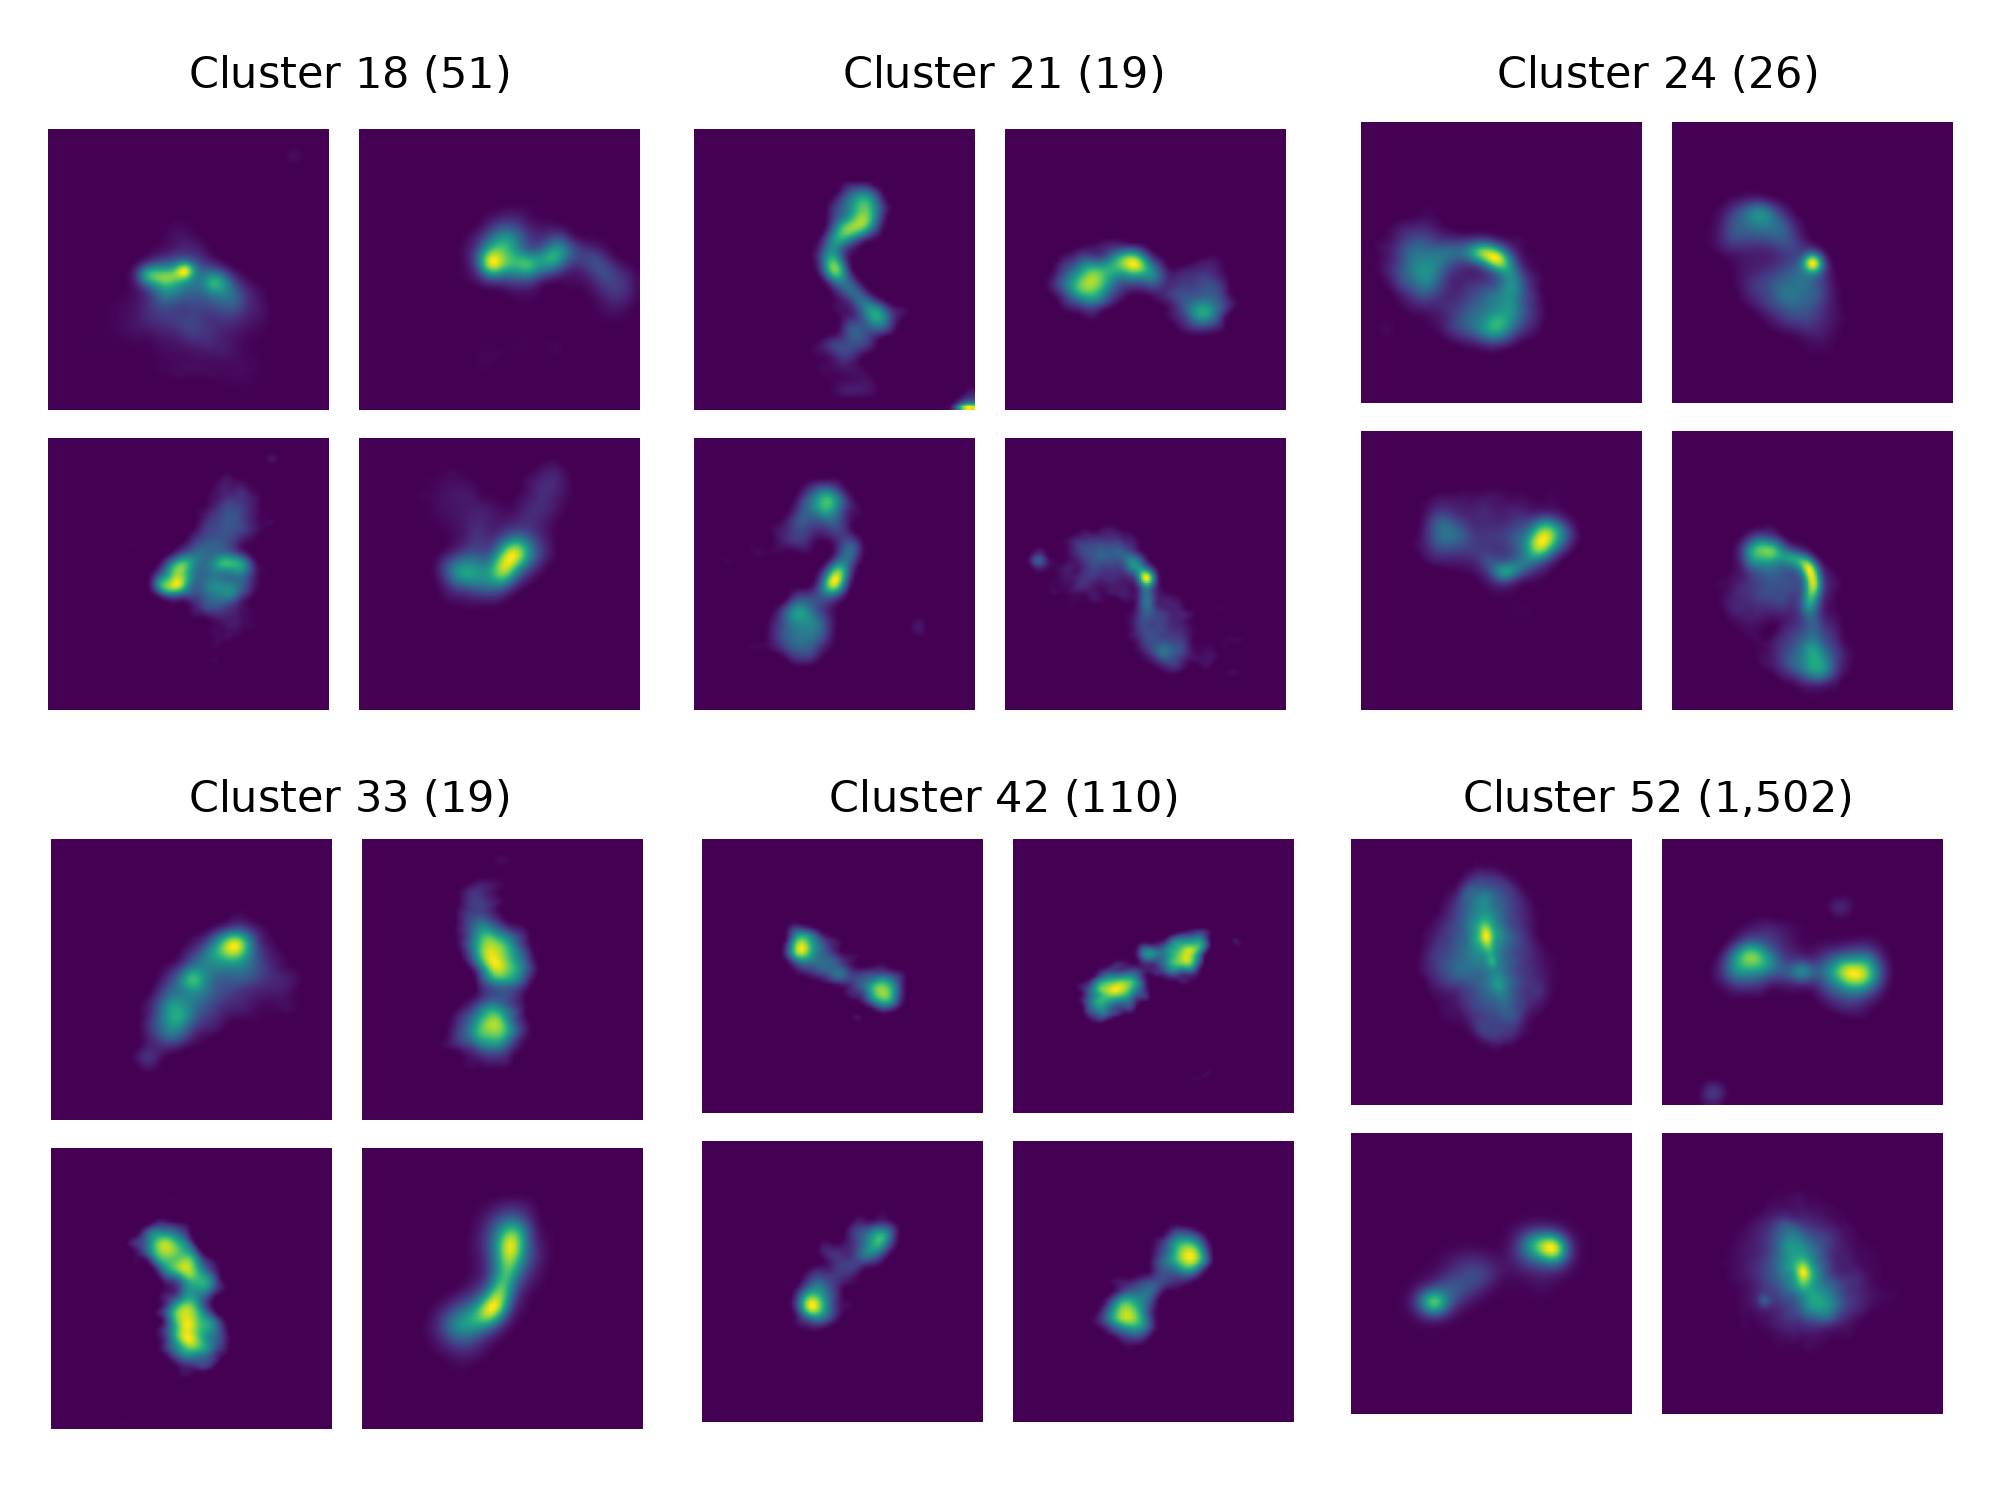
\includegraphics[width=0.85\linewidth]{img/hdbscan_cluster_examples.png}
  \caption[Examples of six raw HDBSCAN clusters]{Six raw HDBSCAN clusters. The headings are the original HDBSCAN labels with the total membership of each cluster.}
  \label{fig:hdbscan_cluster_examples}
\end{figure}

\subsection{Cluster-based class construction}
\label{sec:method_labels}

At this stage, we derive the internal taxonomy from the clustered representations that form the basis of the labels used to fine-tune the classifier.

First, each raw cluster is inspected visually. Clusters representing the same visual morphology are merged,
while clusters unsuitable for the internal taxonomy are returned to the unassigned pool.
This consolidation assigns \(3\,456\) sources to the eleven morphology classes defined below:
\begin{itemize}[leftmargin=*]
\item \textbf{Amorphous:} diffuse, extended emission without clearly defined jets, lobes, or hotspots.
\item \textbf{Asymmetric core-jet (ACJ):} a bright central component with predominantly one-sided extended emission.
\item \textbf{Bright-core:} compact, centrally peaked emission dominated by a bright core, with faint or absent extended structure.
\item \textbf{Centre-bright (FRI):} two-sided, FRI-like emission concentrated towards the centre and fading outwards.
\item \textbf{Core-Displaced:} extended emission containing a dominant compact component offset from the centroid of the resolved structure.
\item \textbf{Edge-bright (FRII) linear:} approximately collinear, FRII-like emission with brightness peaks near the outer edges.
\item \textbf{Hybrid (FRX) unclear:} mixed or ambiguous brightening patterns that do not admit a clear FRI or FRII assignment.
\item \textbf{Large FRII:} large-angular-extent, edge-bright FRII-like emission.
\item \textbf{Spirals:} extended disc- or spiral-like radio emission rather than a jet-and-lobe morphology.
\item \textbf{Structured-Bent:} resolved multi-component emission following a curved or bent axis.
\item \textbf{Unresolved:} point-like or marginally resolved emission in the normalised cutout.
\end{itemize}
These classes are operational descriptions of appearance in the normalised LoTSS-DR2 cutouts and do not constitute independently verified physical classifications.

Next, to reduce the propagation of atypical cluster members into the classifier, we compute the mean SI-SSIM of each source relative to the other members of its assigned class.
Figure~\ref{fig:class_grid} shows the seven highest-ranked sources in each class before filtering, together with their mean SI-SSIM values.
The most mutually similar \(80\,\%\) are retained by default, with class-specific retention fractions between \(60\) and \(90\,\%\) selected according to visual homogeneity.
The resulting labelled subsample is presented in Table~\ref{tab:labelled_subsample}.
The class-balanced split, shared by all ensemble members, assigns \(2\,602\), \(22\) and \(33\) sources to training, validation and testing, respectively.
The smallest class is divided approximately \(70/15/15\). Every larger class contributes the same numbers of validation and test sources, with all remaining members used for training. This produces class-balanced validation and test sets, although their small sizes prevent reliable estimation of per-class performance.
The validation and test sources also participated in self-supervised pre-training.
Sources outside the labelled subsample enter the classifier only during inference (Sec.~\ref{sec:results_classification}).

\begin{table}[H]
\centering
\begin{tabular}{lrr}
\toprule
Class & Sources & Retained (\%) \\
\midrule
Amorphous & 17 & 80 \\
Asymmetric core-jet (ACJ) & 38 & 80 \\
Bright-core & 946 & 80 \\
Centre-bright (FRI) & 267 & 80 \\
Core-Displaced & 16 & 80 \\
Edge-bright (FRII) linear & 437 & 80 \\
Hybrid (FRX) unclear & 67 & 90 \\
Large FRII & 72 & 80 \\
Spirals & 96 & 80 \\
Structured-Bent & 268 & 90 \\
Unresolved & 433 & 60 \\
\midrule
Total & 2\,657 & \\
\bottomrule
\end{tabular}
\caption[Labelled subsample and SI-SSIM retention fractions]{Labelled subsample produced by cluster-based label construction: sources retained per class and class-specific SI-SSIM retention fraction.}
\label{tab:labelled_subsample}
\end{table}

Figure~\ref{fig:curated_pca_3d} visualises how the curated morphology classes are arranged within the pre-trained representation space and relative to the unassigned sources.
Their partial concentration shows that the encoder captures morphology-related structure, while overlaps indicate that the first three PCs,
which retain \(48.81\,\%\) of the curated-subset variance, do not fully separate the classes. This descriptive projection was not used for class construction.

\begin{figure}[H]
  \centering
  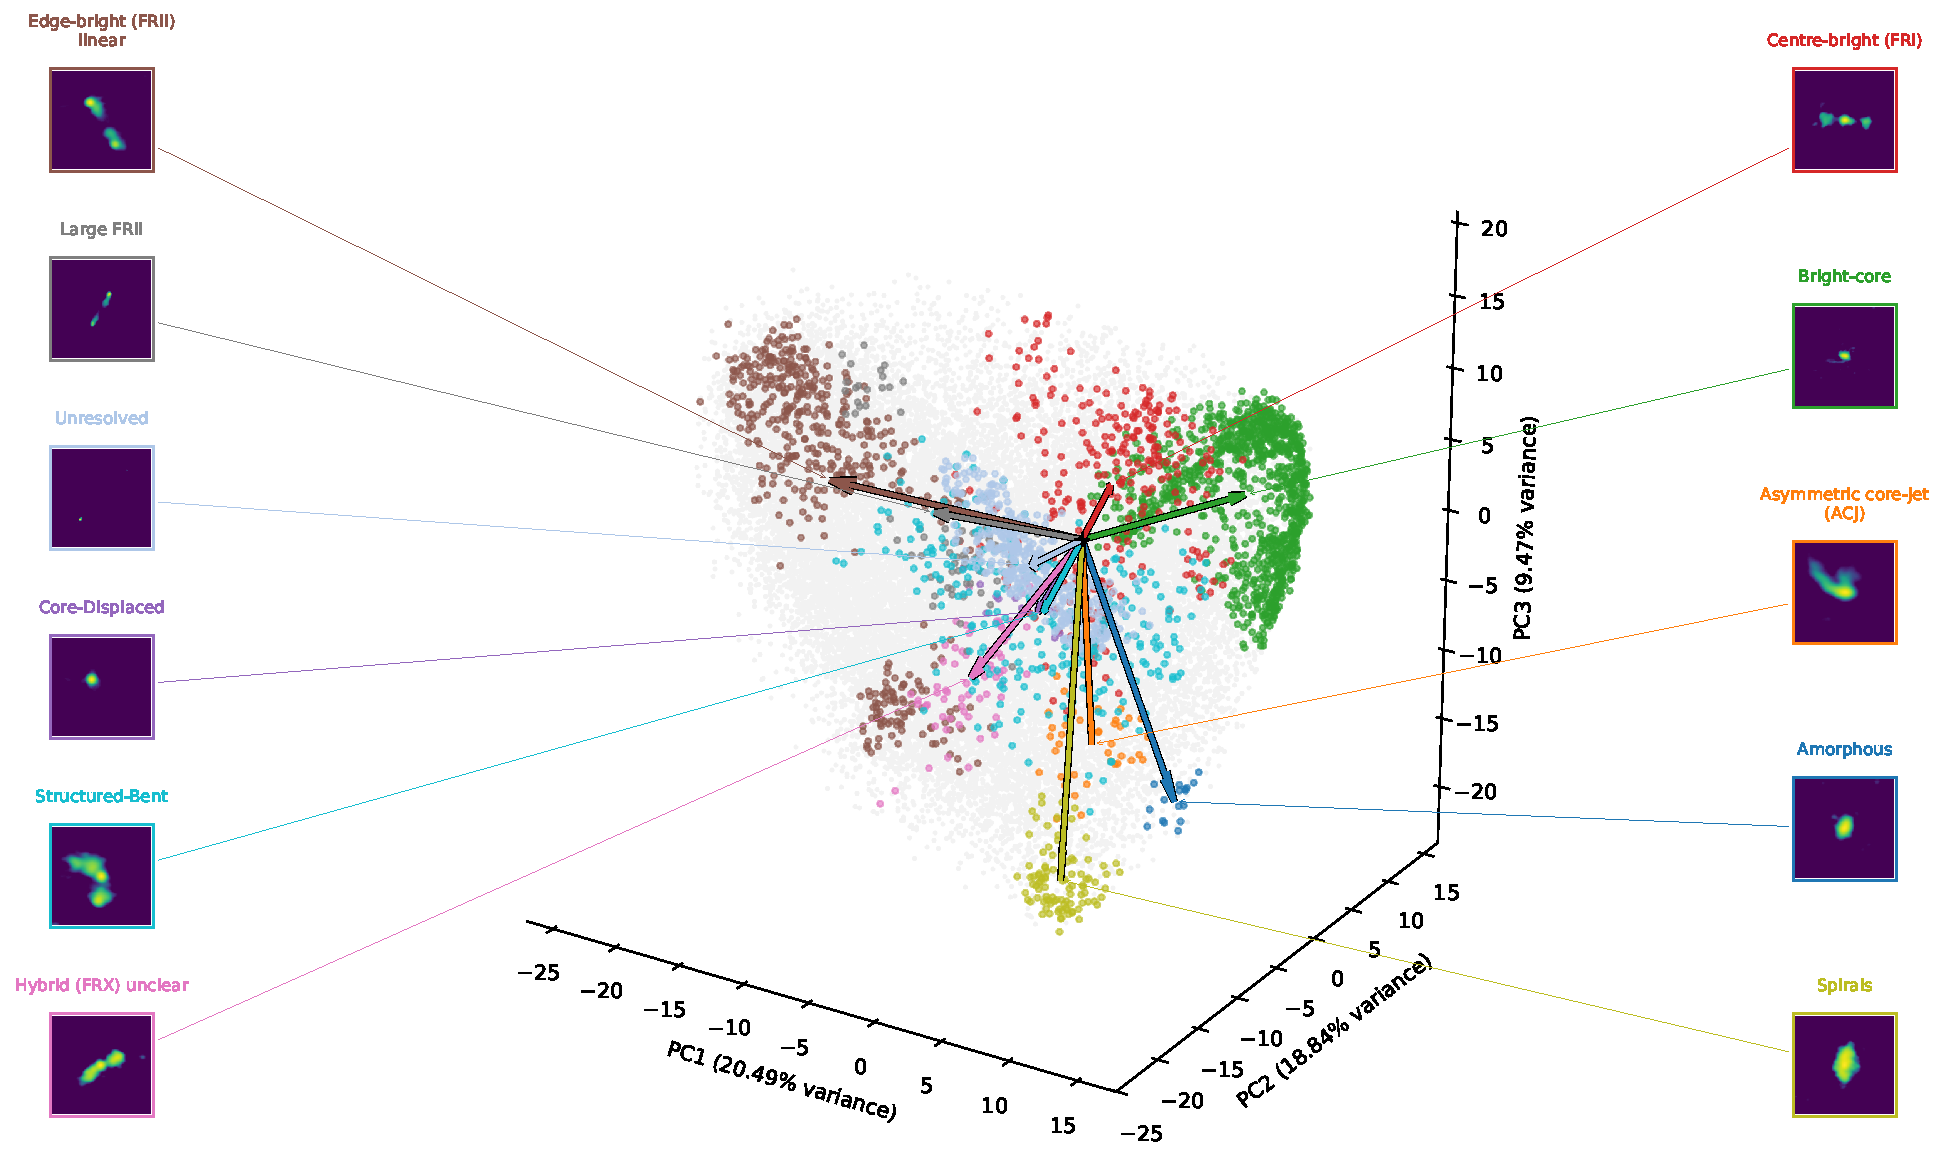
\includegraphics[width=\linewidth]{img/curated_pca_3d.pdf}
  \caption[PCA projection of curated classes and unassigned sources]{Three-dimensional PCA projection of the curated morphology classes
    and unassigned sources.}
  \label{fig:curated_pca_3d}
\end{figure}

\begin{figure}[H]
  \centering
  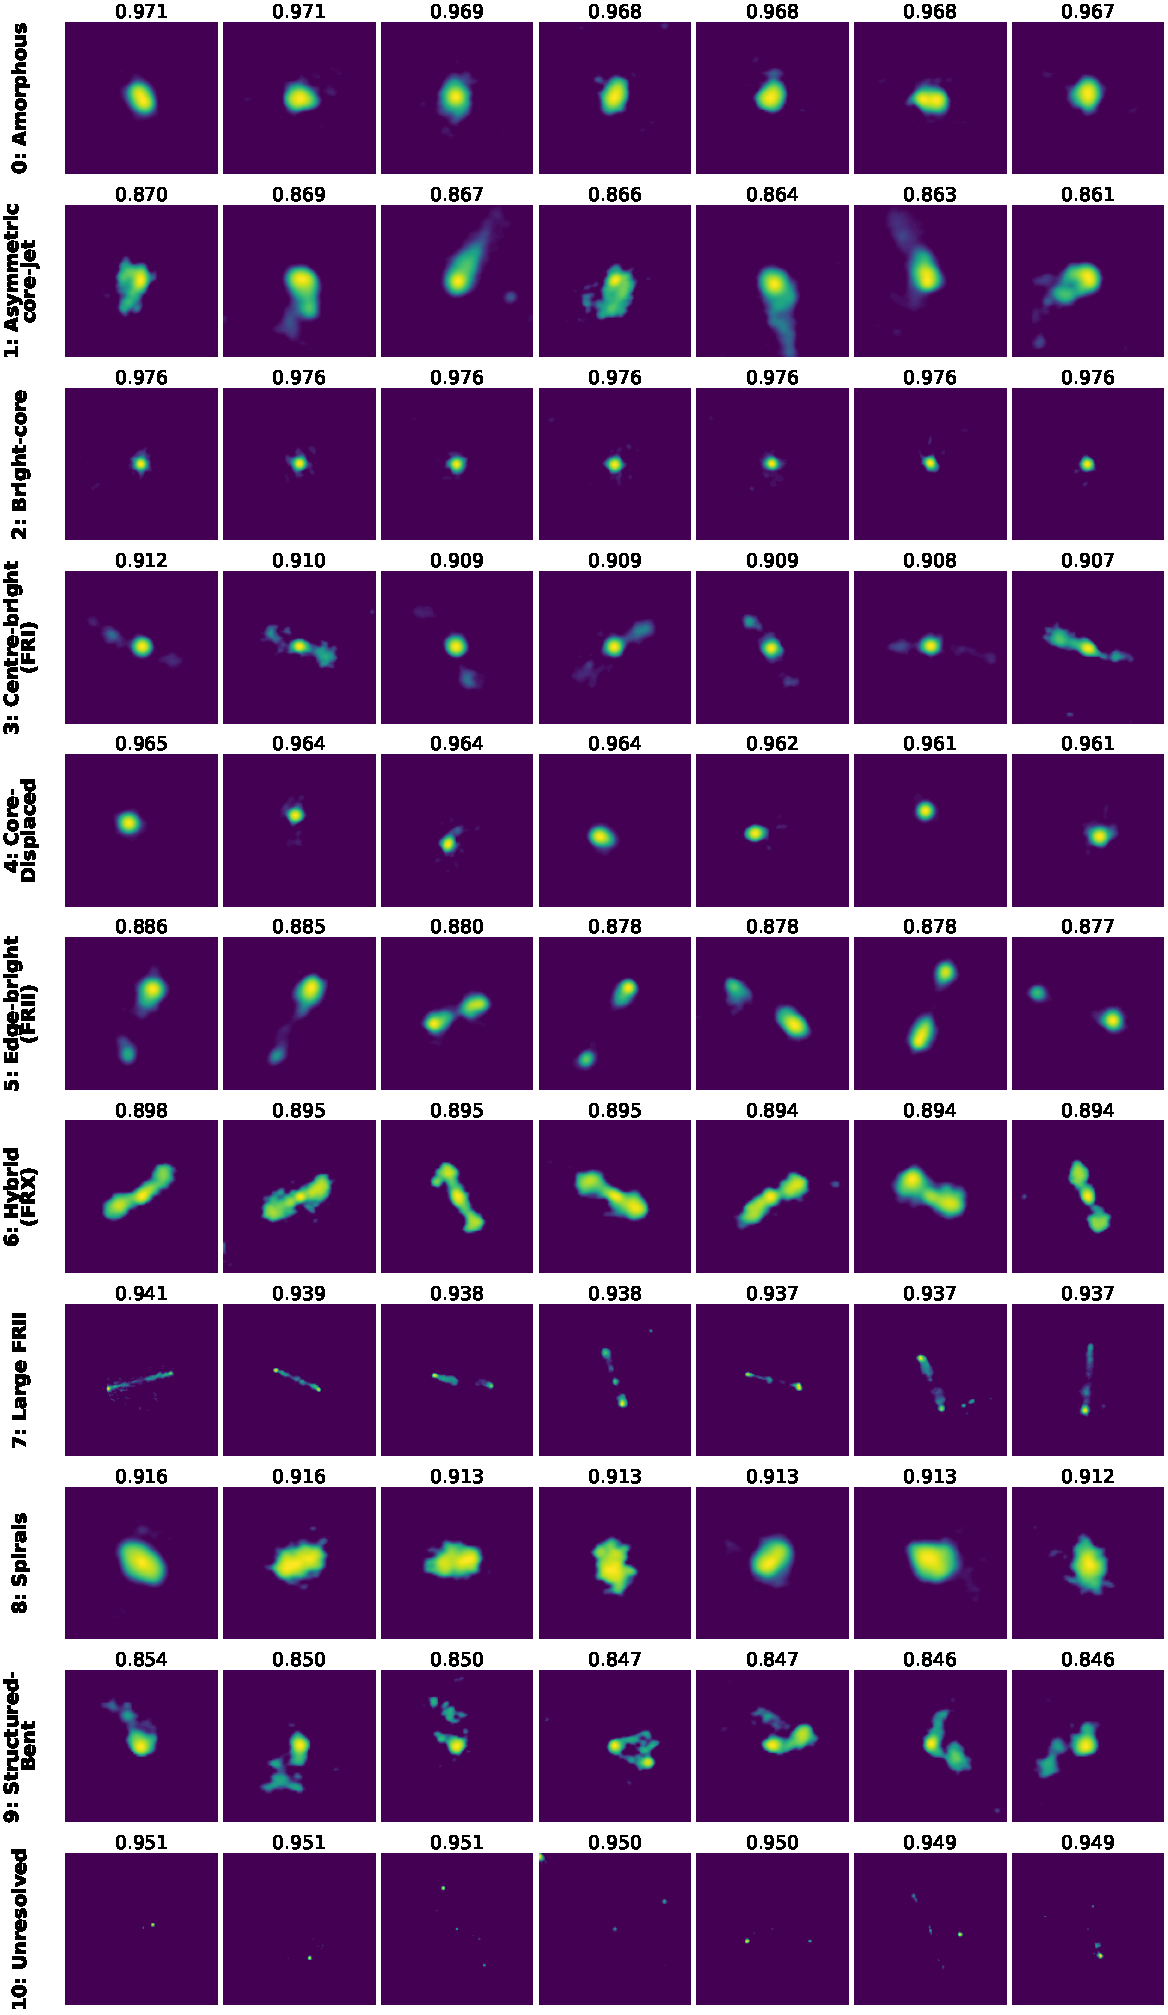
\includegraphics[width=\linewidth,height=0.9\textheight,keepaspectratio]{img/class_grid.pdf}
  \caption[Examples of the eleven internal morphology classes]{Representative LoTSS-DR2 cutouts for the eleven morphology classes.
    Each row shows the seven pre-filter sources with the highest mean within-class SI-SSIM.}
  \label{fig:class_grid}
\end{figure}

\subsection{Supervised classifier and deep ensemble}
\label{sec:method_classifier}

At this stage, with the curated morphology classes already defined, the projector is discarded and a classification head is attached to the pre-trained encoder.
The classifier maps the \(512\)-dimensional representation to eleven class logits\footnote{Unnormalised class scores converted to probabilities by the softmax function.}. We fine-tune both the encoder and the head on the labelled subsample.

The fine-tuning loss function (for a minibatch of \(B\) sources) combines two terms:
\begin{itemize}
\item \textbf{Cross-entropy} loss $\mathcal{L}_{\mathrm{CE}}$, which rewards correct class predictions \citep{Salakhutdinov2007}: 
\begin{equation}
\mathcal{L}_{\mathrm{CE}}
=-\frac{\sum_{i=1}^{B}w_{y_i}\log p_{i,y_i}}
{\sum_{i=1}^{B}w_{y_i}},
\label{eq:classifier_ce}
\end{equation} 
where \(p_{i,y_i}\) is the predicted probability of source \(i\)'s assigned class \(y_i\).
The inverse-frequency weights are \(w_c=N_{\mathrm{train}}/(K n_c)\), with \(N_{\mathrm{train}}\) training sources, \(n_c\) members of class \(c\), and \(K=11\) classes.
\item \textbf{Soft Nearest Neighbour} loss $\mathcal{L}_{\mathrm{SNN}}$, which encourages sources of the same class to have similar representations \citep{Frosst2019}:
\begin{equation}
\mathcal{L}_{\mathrm{SNN}}=-\frac{1}{B}\sum_{i=1}^{B}w_{y_i}\log
\frac{\sum_{j\ne i,\,y_j=y_i}\exp(s_{ij}/\tau_{\mathrm{SNN}})}
{\sum_{j\ne i}\exp(s_{ij}/\tau_{\mathrm{SNN}})},
\label{eq:classifier_snn}
\end{equation}
where \(s_{ij}\) is the cosine similarity between encoder representations, as defined in Sec.~\ref{sec:bg_ssl}. The neighbour sums run over the current minibatch, and the SNN expression assumes at least one same-class neighbour for each source.
\end{itemize}
Thus, the total loss is
\begin{equation}
\mathcal{L} \;=\; \alpha\,\mathcal{L}_{\mathrm{CE}} \;+\; (1-\alpha)\,\mathcal{L}_{\mathrm{SNN}},
\label{eq:ft_loss}
\end{equation}
with \(\alpha=0.5\) and SNN temperature \(\tau_{\mathrm{SNN}}=0.07\).
We train for \(100\) epochs with Adam, a batch size of \(512\), 
and an initial learning rate of \(10^{-3}\), reduced when validation accuracy plateaus.
Training and validation use random rotations within \(\pm180^{\circ}\) and random vertical flips, whereas testing uses unaugmented images. We retain the model with the highest validation accuracy.

Fine-tuning is repeated \(M=50\) times from the same pre-trained encoder checkpoint to construct a deep ensemble \citep{Lakshminarayanan2017}. At inference, we average the members' class-probability vectors for each of the \(32\,514\) catalogue sources. The mean probabilities, agreement \(A\), predictive entropy \(H\), and mutual information \(MI\) defined in Eqs.~\ref{eq:ensmean}--\ref{eq:MI} enter the similarity score detailed in Sec.~\ref{sec:method_srg}. Figure~\ref{fig:ensemble_schematic} summarises this inference path.

\begin{figure}[H]
  \centering
  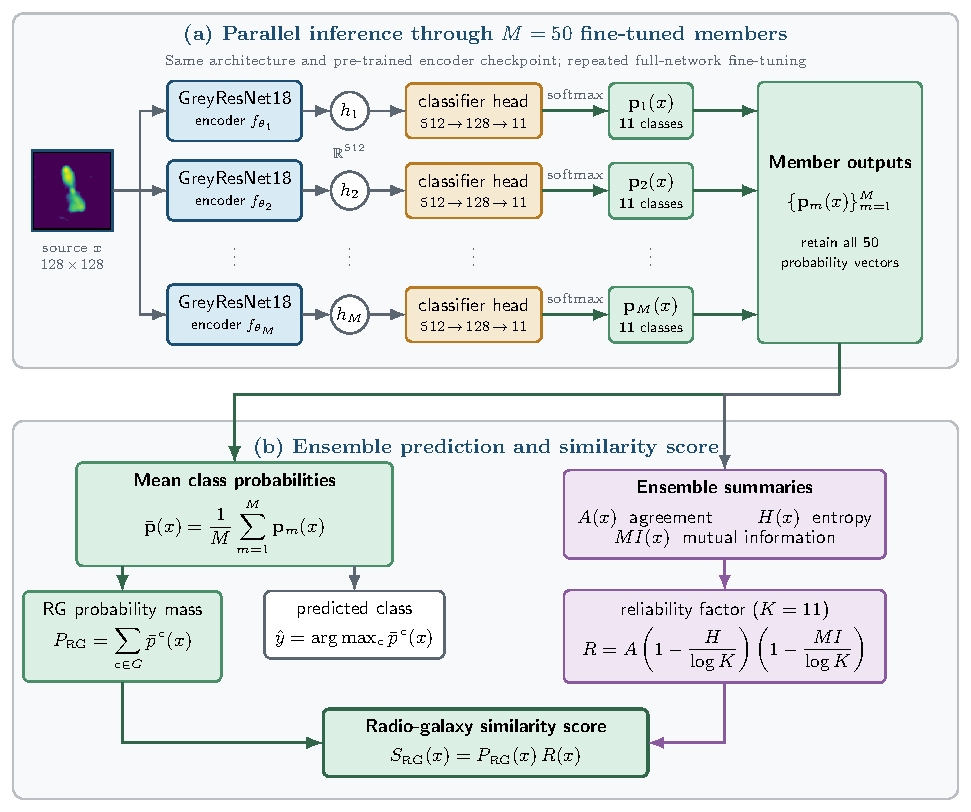
\includegraphics[width=\linewidth]{img/deep_ensemble_schematic.pdf}
  \caption[Deep-ensemble inference and similarity scoring]{Deep-ensemble inference and similarity scoring.}
  \label{fig:ensemble_schematic}
\end{figure}

\subsection{Similarity-to-radio-galaxy score \texorpdfstring{$S_\mathrm{RG}$}{S\_RG}}
\label{sec:method_srg}

Since the primary objective is not to reproduce a fixed external taxonomy but to quantify how strongly a source resembles the radio-galaxy morphologies represented by the model, we group the internal classes into \textit{radio-galaxy-like} (\(G\)) and \textit{non-target} (\(N\)) sets.

Using the internal model labels, the radio-galaxy-like set is defined as
\[
\begin{aligned}
G=\{&\text{Asymmetric core-jet (ACJ)},\\
	&\text{Bright-core},\\
	&\text{Centre-bright (FRI)},\\
	&\text{Core-Displaced},\\
	&\text{Edge-bright (FRII) linear},\\
	&\text{Hybrid (FRX) unclear},\\
	&\text{Large FRII},\\
	&\text{Structured-Bent}\},
\end{aligned}
\]
and the complementary set is
\[
N=\{\text{Amorphous},\ \text{Spirals},\ \text{Unresolved}\}.
\]

We define these groups operationally from the chosen visual classes, including core-dominated appearances in \(G\). Visual inspection of the optical overlays showed that the majority of the sources in the Spirals class are disc galaxies that exhibit radio emission associated with the galactic disc. Amorphous sources lack sufficiently distinct structure for this target, and Unresolved sources provide insufficient spatial information; either class may still contain physical radio galaxies.
This grouping leads to the definition of the radio-galaxy probability mass \(P_\mathrm{RG}\).
With \(\mathbf{p}_m(x)\) denoting the probability vector predicted for source \(x\) by ensemble member \(m\), as introduced in Eq.~\ref{eq:ensmean}, the radio-galaxy probability mass is
\begin{equation}
P_\mathrm{RG}(x)=\sum_{c\in G}\bar{p}^{\,c}(x), \qquad P_\mathrm{RG}(x)\in[0,1].
\label{eq:rg_prob_mass}
\end{equation}

This term measures only how much ensemble-mean probability is assigned to radio-galaxy-like classes.
It does not capture the concentration of the probability vector or the consistency of the member predictions.
Therefore, three complementary summaries -- model agreement \(A(x)\) (Eq.~\ref{eq:ensmean}), predictive entropy \(H(x)\) (Eq.~\ref{eq:H}), and mutual information \(MI(x)\) (Eq.~\ref{eq:MI}) -- are combined into the definition of a reliability factor, 
\begin{equation}
R(x)=A(x)\left(1-\frac{H(x)}{\log K}\right)\left(1-\frac{MI(x)}{\log K}\right).
\label{eq:reliab_factor}
\end{equation}

Dividing \(H\) and \(MI\) by \(\log K\) normalises them by their theoretical maxima for \(K\) classes.
All three factors, and therefore \(R\), lie in the range \([0,1]\).
Hence, the final \textit{similarity-to-radio-galaxy} score is
\begin{equation}
S_\mathrm{RG}(x)=P_\mathrm{RG}(x)\,R(x),\qquad S_\mathrm{RG}(x)\in[0,1].
\label{eq:sim_score}
\end{equation}
For a fixed model and preprocessing pipeline, the score is computed on the same \([0,1]\) scale for every source. Large \(S_\mathrm{RG}\) values indicate strong support for the chosen radio-galaxy-like model classes together with high ensemble consistency.

Fine-class ambiguity also reduces the score when all probability lies within \(G\). If every member assigns \(0.51\) to FRI and \(0.49\) to FRII, then \(P_\mathrm{RG}=A=1\) and \(MI=0\), but \(S_\mathrm{RG}\simeq0.711\). This design favours concentrated support for a particular learned morphology.

\begin{wraptable}{r}{0.40\textwidth}
\begin{minipage}{\linewidth}
\centering
\small
\setstretch{1}
\begin{tabular}{lrrr}
\toprule
 & \(A\) & \(H\) & \(MI\) \\
\midrule
\(A\)  & 1.00 & -0.62 & -0.52 \\
\(H\)  & -0.62 & 1.00 & 0.49 \\
\(MI\) & -0.52 & 0.49 & 1.00 \\
\bottomrule
\end{tabular}
\footnotesize
\caption[Correlations between ensemble reliability measures]{Empirical Pearson correlations between the reliability terms used in \(R(x)\), computed from the classified LoTSS-DR2 catalogue. }
\label{tab:reliability_corr}
\end{minipage}
\end{wraptable}
The reliability terms are empirically correlated (see Table~\ref{tab:reliability_corr}), but they summarise different aspects of the ensemble output. Agreement \(A\) uses only top-class votes, \(H\) measures how broadly the ensemble-mean probability is distributed across classes, and \(MI\) captures disagreement between the members’ probability distributions. Agreement tends to decrease as total or epistemic uncertainty increases, while \(H\) and \(MI\) increase together when ensemble predictions become less stable. Their multiplicative combination is a design choice.
\par
\ifnum\value{WF@wrappedlines}>1
  \vspace{\dimexpr\value{WF@wrappedlines}\baselineskip-\baselineskip\relax}
\fi
\WFclear

\subsection{External catalogue mapping and evaluation}
\label{sec:method_external_mapping}
\label{sec:bg_eval_metrics}

As we discussed in Sec.~\ref{sec:bg_taxonomy}, there is no single universally adopted taxonomy covering all of these morphologies. Therefore, we adopt the morphological correspondences in Table~\ref{tab:morph_mapping} for the comparisons in Sec.~\ref{sec:results_external}, rather than assuming exact equivalence between taxonomies.
In particular, one-sided ridgelines, X-shaped sources, winged sources, and relaxed doubles only approximately correspond to ACJ, Hybrid, Bent, and Amorphous, respectively.
We retain Clews et al.'s uncertain FRI and FRII labels within their respective groups. For external comparison, we combine Edge-bright FRII and Large FRII into a single FRII group.

Clews's one-sided ridgelines are an imperfect ACJ stand-in: inspection of \(100\) examples suggested that only about \(60\,\%\) were genuinely one-sided sources \citep{Clews2025}.
Our ambiguous Hybrid class is also broader than a physical FRI/FRII hybrid or an X-shaped morphology. These mappings support comparisons of related appearances, not interchangeable physical labels.

For Horton's multi-label catalogue, we assign the first class satisfying its conditions in the order FRI, FRII, Spirals, Amorphous, Hybrid, ACJ, then Bent.
Sources satisfying none of these rules remain unmapped; multiple flags do not automatically imply exclusion.

\begin{table}[H]
\centering
\small
\setlength{\tabcolsep}{3pt}
\renewcommand{\arraystretch}{1.15}
\begin{tabular}{@{}p{0.055\linewidth}p{0.16\linewidth}p{0.245\linewidth}p{0.26\linewidth}p{0.22\linewidth}@{}}
\hline
\raggedright Class ID & Class name & \raggedright\citet{Clews2025} & \raggedright\citet{Horton2025} & \citet{Chilufya2025}\\
\hline
0 & Amorphous & -- & \texttt{relaxed}$^a$, \texttt{diffuse}$^a$ & relaxed \\ \hline
1 & ACJ & one\_sided\_ridge & \texttt{onesided} & -- \\ \hline
2 & Bright-core & -- & -- & -- \\ \hline
3 & FRI & FRI, uncertain\_FRI & \texttt{fri}$^b$ & FRI \\ \hline
4 & Core-Displaced & -- & -- & -- \\ \hline
5 & FRII & FRII, uncertain\_FRII & \texttt{frii}$^b$ & FRII \\ \hline
6 & Hybrid & -- & \texttt{hybrid}, \texttt{xshaped} & -- \\ \hline
7 & Large FRII & -- & -- & -- \\ \hline
8 & Spirals & -- & \texttt{spiral} & -- \\ \hline
9 & Bent & bent & \raggedright \texttt{cshaped}$^a$, \texttt{sshaped}$^a$, \texttt{wings}$^a$ & WAT, NAT, headtail \\ \hline
10 & Unresolved & -- & -- & -- \\
\hline
\multicolumn{5}{@{}p{\linewidth}@{}}{Unmapped: Clews -- \textit{other}, \textit{triple}; Horton -- no mapping rule satisfied.} \\
\hline
\multicolumn{5}{@{}p{\linewidth}@{}}{\footnotesize $^a$ Only when \texttt{fri} and \texttt{frii} are both false.} \\
\multicolumn{5}{@{}p{\linewidth}@{}}{\footnotesize $^b$ Only when the other FR flag is false (exclusive).} \\
\end{tabular}
\caption[Mapping between external and internal morphology classes]{Adopted morphological correspondences between reference catalogues and our internal classes.
A dash (--) indicates that no direct mapping is adopted.}
\label{tab:morph_mapping}
\end{table}

For each external-catalogue comparison, the target morphology defines the positive class and the remaining mapped morphologies define the negative class.
A true positive (\(\mathrm{TP}\)) or true negative (\(\mathrm{TN}\)) agrees with the reference assignment. 
A false positive (\(\mathrm{FP}\)) is predicted positive but is negative in the reference, while a false negative (\(\mathrm{FN}\)) is predicted negative but is positive in the reference.
These four counts form the confusion matrix. Precision measures the purity of the predicted positive sample, whereas recall measures the completeness of the positive class:
\begin{equation}
\mathrm{precision}=\frac{\mathrm{TP}}{\mathrm{TP}+\mathrm{FP}},\qquad
\mathrm{recall}=\frac{\mathrm{TP}}{\mathrm{TP}+\mathrm{FN}}.
\end{equation}
The \(F_1\) score combines precision and recall through their harmonic mean,
\begin{equation}
F_1=2\,\frac{\mathrm{precision}\,\mathrm{recall}}{\mathrm{precision}+\mathrm{recall}}.
\end{equation}

A higher \(F_1\) score indicates better classification performance on the evaluated sample.

We estimate uncertainty in the reported metrics from the number of evaluated sources and repeated resampling of each comparison sample. The resulting bounds describe how the metrics may vary with sample membership -- label errors, selection bias and training variability require separate assessment.
Each catalogue is evaluated separately, with calculation details in Appendix~\ref{app:evaluation}.

We also repeat the comparisons after excluding all \(2\,657\) curated sources, across angular-size ranges, and without Clews's uncertain FR labels. Excluding curated sources removes overlap with supervised training, although the remaining sources still participated in pre-training.

\subsection{Application to diffuse radio emission}
\label{sec:method_relics}

We used the selected radio relics described in Sec.~\ref{sec:data_relics} to test the trained ensemble on diffuse radio emission.
The aim is to examine how their morphology is represented by the radio-galaxy classifier. 
Bright radio galaxies within a relic cutout can dominate the normalised input, while clipping can suppress the relic's low-surface-brightness emission.
We therefore mask neighbouring sources before preprocessing to focus the test on the diffuse emission.

We start with relic-centred LoTSS-DR3 cutouts with a side length of \(1.5\times\mathrm{LAS}\). Then, we manually draw polygonal regions around the relic emission, exclude pixels outside them, estimate the sigma-clipped standard deviation \(\sigma\) from the retained pixels and then set both masked pixels and values below \(3\sigma\) to this floor. The images are resampled to \(128\times128\) pixels and min--max normalised for inference.

These selected examples illustrate the model's response to isolated relic emission, rather than its performance on unmasked fields. The assigned labels describe resemblance to the learned classes.
